
\chapter{Some Important Hints to Work with \LaTeX\ }\label{sec:latexenv}

This section describes some sample codes for often used elements in \LaTeX.

\section{Structure}\label{sec:structure}

A text can be structured with the commands \texttt{\textbackslash
chapter\{.\}}, \texttt{\textbackslash section\{.\}},
\texttt{\textbackslash subsection\{.\}} and \texttt{\textbackslash
subsubsection\{.\}}.

\section{References and Citations}\label{sec:refverw}

Literature references are created with the command  \texttt{\textbackslash
cite\{.\}}. An example: \cite{mahony2005complementary}.

The command \texttt{\textbackslash footnote\{.\}} can be used to create a footnote.
An footnote example\footnote{This is the text in my footnote.}.

To make cross references the command \texttt{\textbackslash label\{.\}} is used to pin the reference and the command \texttt{\textbackslash ref\{.\}}  to refer to the reference.
An example reference to the second chapter: chapter~\ref{sec:latexenv}.


\section{Itemization}\label{sec:item}

The following itemization example without enumeration,
\begin{itemize}
  \item point 1
  \item point 2
\end{itemize}
was constructed with:
\begin{verbatim}
\begin{itemize}
  \item point 1
  \item point 2
\end{itemize}
\end{verbatim}

The following itemization example with enumeration,
\begin{enumerate}
  \item point 1
  \item point 2
\end{enumerate}
was constructed with:
\begin{verbatim}
\begin{enumerate}
  \item point 1
  \item point 2
\end{enumerate}
\end{verbatim}

The following itemization example,
\begin{description}
  \item[P1] point 1
  \item[P2] point 2
\end{description}
was constructed with:
\begin{verbatim}
\begin{description}
  \item[P1] point 1
  \item[P2] point 2
\end{description}
\end{verbatim}


\section{How to Create a Table}\label{sec:tables}

A table example:
\begin{table}[h]
\begin{center}
 \label{tab:tabnefz}
 \begin{tabular}{ll|ccc}
 \hline
  & Unit & ECE & EUDC & NEFZ \\ \hline \hline
 Time & s & 780 & 400 & 1180 \\
 Distance & km & 4.052 & 6.955 & 11.007 \\
 Average velocity & km/h & 18.7 &  62.6 & 33.6 \\
 Idle running & \% & 36 & 10 & 27 \\
 \hline
 \end{tabular}
 \caption{Data of driving cycles ECE, EUDC, NEFZ.}
\end{center}
\end{table}

The table was created with the following code:
\begin{verbatim}
\begin{table}[h]
\begin{center}
 \label{tab:tabnefz}
 \begin{tabular}{ll|ccc}
 \hline
  & Unit & ECE & EUDC & NEFZ \\ \hline \hline
 Time & s & 780 & 400 & 1180 \\
 Distance & km & 4.052 & 6.955 & 11.007 \\
 Average velocity & km/h & 18.7 &  62.6 & 33.6 \\
 Idle running & \% & 36 & 10 & 27 \\
 \hline
 \end{tabular}
 \caption{Data of driving cycles ECE, EUDC, NEFZ.}
\end{center}
\end{table}
\end{verbatim}


\section{Include a Vectorized Graphic}\label{sec:pdfgraph}

With the following command lines one can include a pdf graphic:
\begin{verbatim}
\begin{figure}[h]
   \centering
   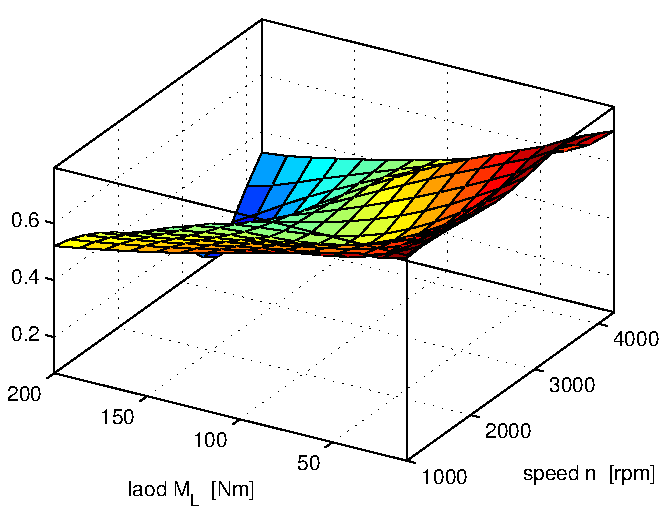
\includegraphics[width=0.75\textwidth]{pics/k_surf.pdf}
   \caption{A picture.}
   \label{pics:k_surf}
\end{figure}
\end{verbatim}

\begin{figure}[h]
   \centering
   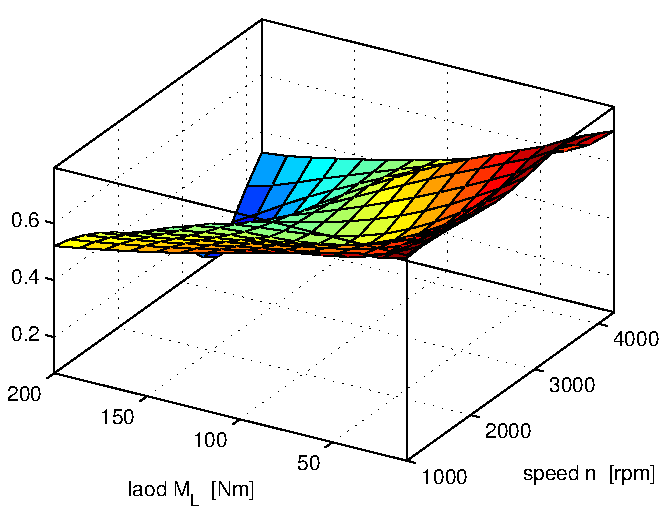
\includegraphics[width=0.75\textwidth]{pics/k_surf.pdf}
   \caption{A picture.}
   \label{pics:k_surf}
\end{figure}

or two pictures next to each other:
\begin{verbatim}
\begin{figure}[h]
  \begin{minipage}[t]{0.48\textwidth}
    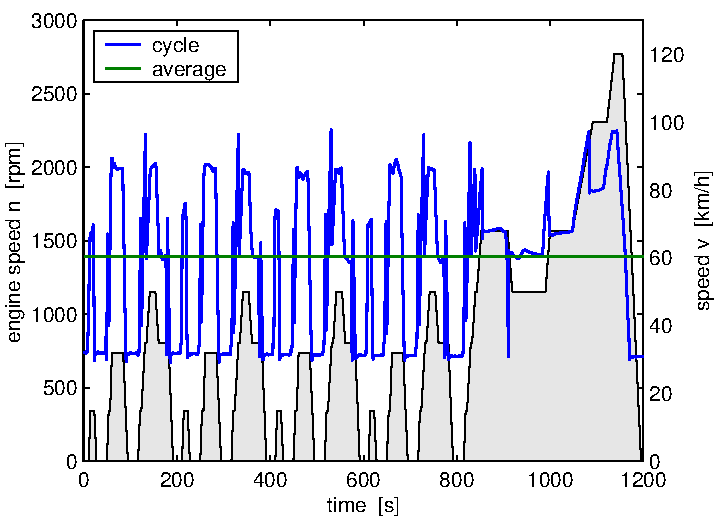
\includegraphics[width = \textwidth]{pics/cycle_we.pdf}
  \end{minipage}
  \hfill
  \begin{minipage}[t]{0.48\textwidth}
    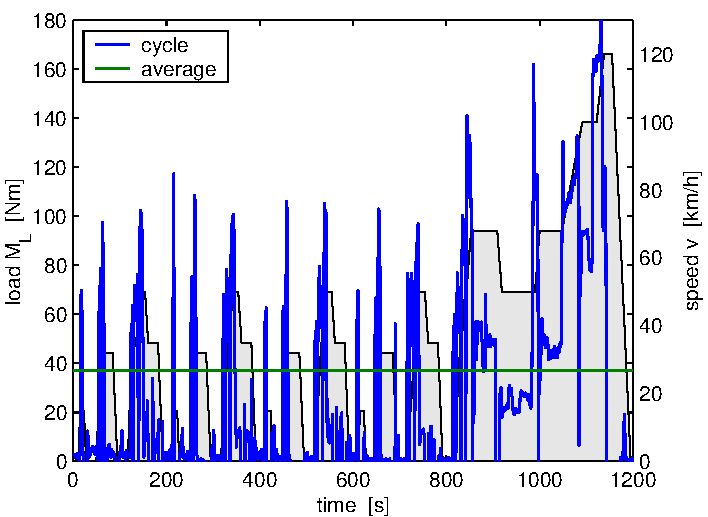
\includegraphics[width = \textwidth]{pics/cycle_ml.pdf}
  \end{minipage}
  \caption{Two pictures next to each other.}
  \label{pics:cycle}
\end{figure}
\end{verbatim}

\begin{figure}[h]
  \begin{minipage}[t]{0.48\textwidth}
    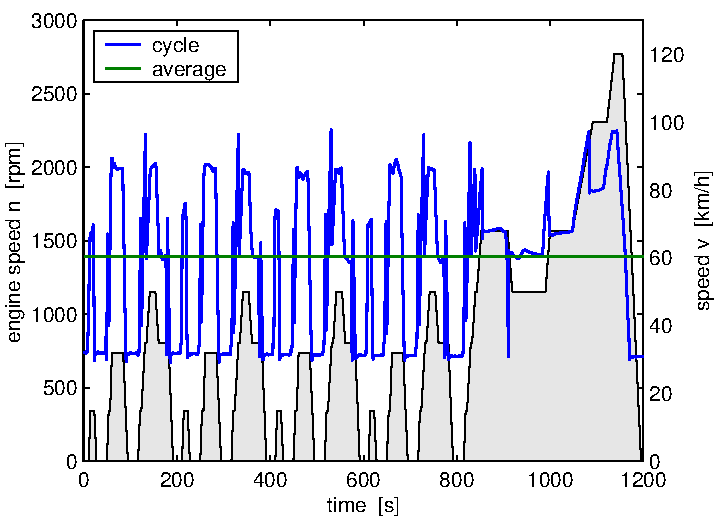
\includegraphics[width = \textwidth]{pics/cycle_we.pdf}
  \end{minipage}
  \hfill
  \begin{minipage}[t]{0.48\textwidth}
    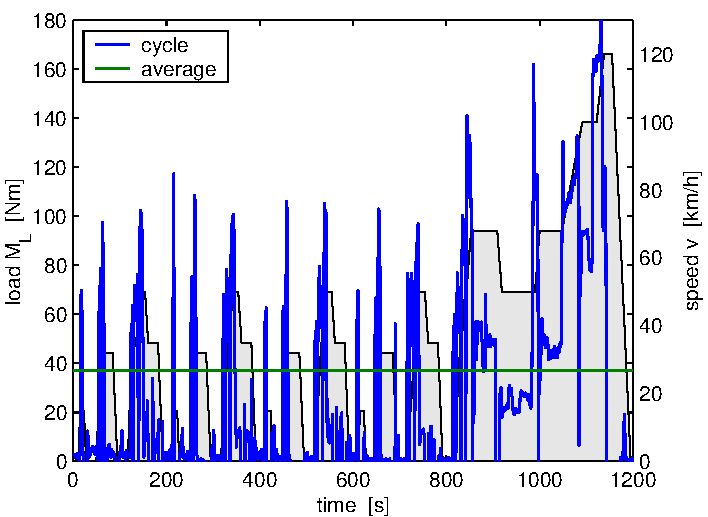
\includegraphics[width = \textwidth]{pics/cycle_ml.pdf}
  \end{minipage}
  \caption{Two pictures next to each other.}
  \label{pics:cycle}
\end{figure}

Note: By replacing the positioning parameter \texttt{h} by \texttt{H} the position of the graphic can be controlled.

\section{Mathematical Formulas}\label{sec:math}

In the equation environment one can type very easily mathematical equations.
\begin{equation}
 p_{me0f}(T_e,\omega_e) \ = \ k_1(T_e) \cdot (k_2+k_3 S^2
 \omega_e^2) \cdot \Pi_{max} \cdot \sqrt{\frac{k_4}{B}} \, .
\end{equation}

The code for this example:
\begin{verbatim}
\begin{equation}
 p_{me0f}(T_e,\omega_e) \ = \ k_1(T_e) \cdot (k_2+k_3 S^2
 \omega_e^2) \cdot \Pi_{max} \cdot \sqrt{\frac{k_4}{B}} \, .
\end{equation}
\end{verbatim}

Some other examples:
\[
z \left( 1 \ +\ \sqrt{\omega_{i+1} + \zeta -\frac{x+1}{\Theta +1} y + 1} 
\ \right)
\ \ \ =\ \ \ 1
\]


\begin{equation}
\left[
{\bf X} + {\rm a} \ \geq\ 
\underline{\hat a} \sum_i^N \lim_{x \rightarrow k} \delta C
\right]
\end{equation}

One can also create mathematical expressions in the text with \$my equation\$ (e.g. $a^2+b^2=c^2$).
\newline

Or let's place a 6 by 6 matrix:
\begin{equation}\label{MeineMatrix}
    \begin{pmatrix}
      1 & 0 & 0 & 0 & 0 & 0 \\
      0 & 1 & 0 & 0 & 0 & 0 \\
      0 & 0 & 1 & 0 & 0 & 0 \\
      0 & 0 & 0 & 1 & 0 & 0 \\
      0 & 0 & 0 & 0 & 1 & 0 \\
      0 & 0 & 0 & 0 & 0 & 1 \\
    \end{pmatrix}
\end{equation}

The code to create this matrix:
\begin{verbatim}
\begin{equation}\label{MeineMatrix}
    \begin{pmatrix}
      1 & 0 & 0 & 0 & 0 & 0 \\
      0 & 1 & 0 & 0 & 0 & 0 \\
      0 & 0 & 1 & 0 & 0 & 0 \\
      0 & 0 & 0 & 1 & 0 & 0 \\
      0 & 0 & 0 & 0 & 1 & 0 \\
      0 & 0 & 0 & 0 & 0 & 1 \\
    \end{pmatrix}
\end{equation}
\end{verbatim}



\section{Other Useful Commands}\label{sec:div}

 \emph{Emphases} in the text can be created with the command \texttt{\textbackslash epmh\{.\}}.
Between the commands \text{\textbackslash begin\{verbatim\}} and  \text{\textbackslash begin\{verbatim\}} you can write text which is not compiled from LaTeX like \begin{verbatim} \section{My new section} or \chapter{Chapter 2} or \emph{italic?}\end{verbatim}.
